\documentclass[10pt]{article}
\usepackage[T1]{fontenc}
\usepackage[
    papersize={9in, 12in}, left=0.25in, right=0.75in, top=0.75in]{geometry}
\usepackage{array, booktabs, fontspec, nopageno, xfrac, xltxtra, xunicode}
\usepackage{hanging}
\usepackage[factor=2000]{microtype}
\setmainfont{Adobe Garamond Pro}
\begin{document}

\begin{center}

{\huge \textsc{Playing Techniques}}

\end{center}

\vspace*{1\baselineskip}

\newcolumntype{V}{>{\centering\arraybackslash} m{2cm} }
\newcolumntype{W}{>{\centering\arraybackslash} m{6cm} }
\renewcommand{\arraystretch}{2}
\begin{tabular}[t]{Vm{7cm}}
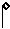
\includegraphics{../_assets/natural-harmonic.pdf}
    &
    natural harmonic;
    open diamonds even for black-note durations.
    \\

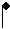
\includegraphics{../_assets/half-harmonic.pdf}
    &
    \hangpunct{
    ``half-harmonic'' finger pressure;
    filled diamonds even for white-note durations.
    }
    \\

\textbf{$\sfrac{1}{2}$ clt}
    &
    col legno / coi crini tratto:
    rotate wrist;
    draw bow across string with wood and hair at same time;
    faster bowstrokes give distinctive whisking.
    \\

\textbf{clicks}
    &
    individuated clicks of \textit{extremely} slow bow passing over string;
    exact rhythm not controlled;
    follow density indications given in score.
    \\

\textbf{scr.}
    &
    scratch tone;
    use very slow bow;
    suppress subtones at loud dynamics;
    encourage flickering intermittency at quiet dynamics.
    \\
\end{tabular}
%
\begin{tabular}[t]{Vm{7cm}}
\textbf{spazz.}
    &
    spazzolato:
    sweep bow repeatedly up and down string in $\sfrac{1}{2}$ clt position;
    also `spz.'
    \\

\textbf{RH vib.}
    &
    RH `vibrato':
    shake or jostle bow with RH during bowstroke;
    resultant sound not controllable like ordinary LH vibrato;
    aim for wobble or perturbation in sound.
    \\

\textbf{XFB}
    & 
    \hangpunct{
    ``extremely fast bow'': very pronounced flautando;
    play with generous amounts of bow lightly skimming the string;
    resulting color almost `fluorescent';
    prolong the color with irregular retakes of the bow;
    only occurs at quiet dynamics.
    }
    \\

\end{tabular}

\vspace*{2.5\baselineskip}

\renewcommand{\arraystretch}{2.5}
\begin{tabular}[t]{Wm{8cm}}
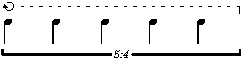
\includegraphics{../_assets/circle.pdf}
    &
    circle bow;
    one complete circle per duration;
    five circles shown here.
    \\

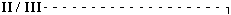
\includegraphics{../_assets/cross-string.pdf}
    &
    cross-string bow tremolo;
    exactly equivalent to conventional slur-plus-tremolo notation
    in music of common practice;
    always appears over double stop (here II and III);
    indicated verbally here to afford performer choice in exact
    rhythm of alternation between pitches.
    \\

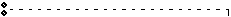
\includegraphics{../_assets/double-diamond.pdf}
    &
    \hangpunct{
    ``two-finger harmonic'':
    lay two fingers lightly on string;
    resultant sound highly unpredicatble
    though frequently `dirty' harmonic.
    }
    \\ 

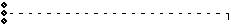
\includegraphics{../_assets/triple-diamond.pdf}
    &
    \hangpunct{
    ``three-finger harmonic'':
    lay three fingers lightly on string;
    pitch still present but strongly veiled;
    exactly equivalent to damp (below).
    }
    \\ 

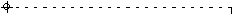
\includegraphics{../_assets/damp.pdf}
    &
    \hangpunct{
    damp:
    exactly equivalent to three-finger harmonic (above).
    }
    \\

\end{tabular}

\vspace*{1.5\baselineskip}

\begin{center}

{\huge \textsc{String Contact Points}}

\end{center}

\renewcommand{\arraystretch}{2}
\begin{tabular}[t]{Vm{8cm}}

\textbf{T} & tasto
    \\

\textbf{P} & ponticello
    \\

\textbf{DZ}
    &
    \hangpunct{
    ``dead zone'': last 1 cm of string closest to bridge (but not yet touching
    bridge); pitch almost (but not completely) effaced.
    }
    \\

\textbf{OB}
    &
    \hangpunct{
    ``on bridge'': bow directly on wood of bridge;
    pitch completely effaced;
    resultant sound gives snowlike whitenoise.
    }
    \\

\end{tabular}

\end{document}
